\section*{Тестовые функции}
\addcontentsline{toc}{subsection}{Тестовые функции}

В качестве тестовой функции для минимизации
использовалась смещённая функция Растригина $R$:

\begin{equation*}
    r = \sum_{i = 1}^{D}(x_i^2 - 10\cos(2 \pi x_i) + 10)
\end{equation*}

\begin{equation*}
    R = r\left(\frac{5.12 (x - o_r)}{100}\right) + 800
\end{equation*}

Вектор параметров $x$ был выбран размера 30.

Было проведено тестирование
аналогично описанному в разделе
Численные эксперименты,
однако не были получены
статистические различия.
Отсутствие эффекта
от оптимизации может
быть объяснено тем,
что служебные функции
выполняются значительно быстрее.

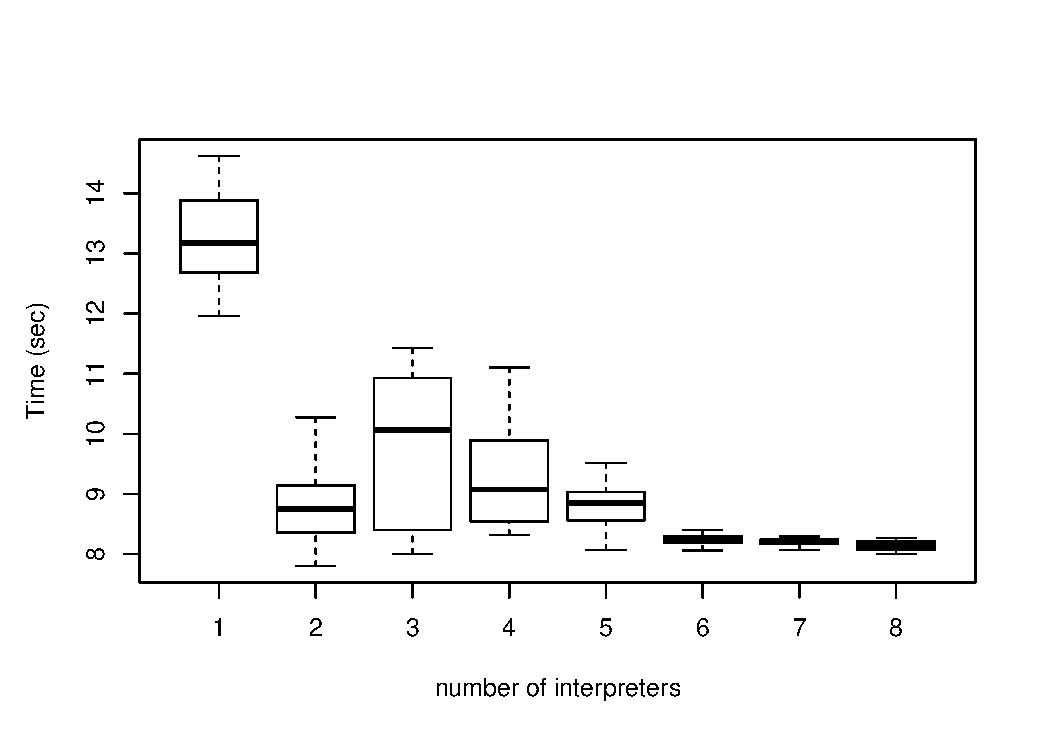
\includegraphics{rastrigin}

На графике видно, что
с увеличением числа интерпретаторов
время работы уменьшается не существенно.

